\section{Resultados}
\label{sec:resultados}

Os resultados dos principais modelos estimados estão na~\hyperref[table:tabela1]{Tabela 1}. Os modelos 1, 2 e 3 são versões do modelo básico: o primeiro utiliza o índice de poder presidencial composto por 14 indicadores; o 2 utilizada apenas três destes indicadores; e o 3 inclui uma variável de efetividade do legislativo. Os modelos 4 e o 5 são regressões binomiais negativas com o número de partidos adicionais como variável dependente

\begin{table}[htb]
\IBGEtab{\caption{Determinantes da ocorrência de coalizões governamentais sobredimensionadas na América Latina, 1979-2012}
\label{table:tabela1}
}{%
\begin{tabular}{lccccc}
\toprule
{} & \textbf{Modelo 1} & \textbf{Modelo 2} & \textbf{Modelo 3} & \textbf{Modelo 4} & \textbf{Modelo 5} \\
\midrule
Número efetivo de partidos & 0.21 & 0.29** & 0.36 & 0.30*** & 0.18** \\
{} & (0.14) & (0.14) & (0.32) & (0.11) & (0.08) \\
Força do legislativo (Polcon3) & 3.55** & 4.19** & 6.56** & 2.86** & 2.65** \\
{} & (1.83) & (2.16) & (3.42) & (1.16) & (1.62) \\
Poder presidencial & 0.04** & & & 0.03*** & \\
{} & (0.02) & & & (0.01)&  \\
Efetividade do legislativo & & & 1.01* & & 1.64*** \\
{} & & & (0.57) & & (0.43) \\
Poder de veto &  & -3.02 & 1.13 & & -4.7** \\
{} &  & (2.11) & (7.32) & & (2.43) \\
Controle do orçamento &  & 0.28 & 0.29 & & -1.82** \\
{} &  & (0.93) & (1.12) &  & (0.88) \\
Decreto legislativo &  & 1.92 & 3.32 & & -0.72 \\
{} & & (1.63) & (3.43) & & (0.98) \\
Extremismo do presidente & -1.15** & -1.3*** & -1.81** & -0.93*** & -0.55** \\
{} & (0.45) & (0.42) & (0.65) & (0.26) & (0.23) \\
Polarização no congresso & -9.06** & -6.63* & -17.06** & -4.93** & -10.63*** \\
{} & (3.82) & (3.52) & (7) & (2.35) & (2.98) \\
Ciclo eleitoral & 1.77** & 1.95** & 2.98** & 0.52* &  0.83*\\
{} & (0.92) & (0.98) & (1.5) & (0.31) & (0.48) \\
\% de cadeiras do presidente & 8.17*** & 9.14*** & 10.83*** & 3.93** & 2.42 \\
{} & (2.7) & (2.97) & (3.82) & (1.58) & (1.6) \\
Inflação_{log} & -0.42* & -0.76** & -1.27** & -0.01** & -0.21*** \\
{} & (0.22) & (0.33) & (0.65) & (0.09) & (0.08) \\
$t$ & -4.47*** & -4.2*** & -3.92*** & & \\
{} & (0.82) & (0.85) & (1.37) & & \\
$t^{2}$ & 0.71*** & 0.64*** & 0.60** & & \\
{} & (0.15) & (0.15) & (0.25)& & \\
$t^{3}$ & -0.03*** & -0.03*** & -0.03** & & \\
{} & (0.01) & (0.01) & (0.1) & & \\
Log-likelihood & -53.14 & -52.29 & -26.47 & -218.12 & -148.72 \\
Clusters & 102 & 102 & 82 & 102 & 82 \\
N & 421 & 421 & 328 & 421 & 328 \\
\bottomrule
\end{tabular}%
}{ %
\nota{$\ast\ast\ast p<0.01; \ast\ast p<0.05; \ast p< 0.1$. Os modelos foram estimados por \textit{maximum likelihood}. Erros-padrão robustos com \textit{cluster} para os presidentes entre parênteses. As constantes foram omitidas e a variável inflação foi atrasada.}
}
\end{table}

Conforme indica a tabela, todos os modelos são consistentes com as hipóteses 1 e 2, e apresentam os sinais esperados em quase todas as variáveis. Congressos capazes de bloquear mudanças no \textit{status quo} e mais fragmentados aumentam a probabilidade de vermos um gabinete sobredimensionado -- ainda que a estimativa do efeito desta  última varie bastante entre os modelos. Inflação elevada, proximidade das eleições e o tamanho da representação do partido do presidente no congresso também apresentam efeitos significantes e condizentes com as expectativas: quando os preços sobem, presidentes perdem popularidade (presume-se) e se tornam menos capazes de administrar coalizões grandes; já no início de seus mandatos, ou quando seus partidos possuem grandes bancadas, o contrário ocorre.

Presidentes mais extremados ideologicamente e congressos mais polarizados diminuem a probabilidade de surgirem grandes coalizões, o que intuitivamente faz sentido: coalizões com partidos próximos ideologicamente são mais fáceis de serem geridas; do mesmo modo, presidentes mais moderados têm menores dificuldades de atrair partidos aos seus gabinetes. A maior surpresa fica por conta da variável que mensura o poder presidencial, que é significativa nos modelos 1 e 4 mas apresenta efeito contrário do que previa a Hipótese 3, isto é, presidentes que contam mais poderes legislativos são \textit{mais} propensos a formar coalizões sobredimensionadas. Verificando o efeito de apenas alguns dos indicadores que de poder presidencial mencionados pela literatura como importantes, entretanto, o modelo 2 mostra que nenhum deles é significativo. Controle do processo orçamentário e poder de expedir decretos apresentam sinais esperados nos modelos 2 e 3, mas não os mantêm nas outras especificações. Por seu turno, o efeito do poder de veto é o mais inconsistente de todos, embora seja significativo e apresente o sinal esperado no modelo 5: de acordo com este, quando possui o poder de evitar mudanças no \textit{status quo} contrárias aos seus interesses, presidentes são menos impelidos à formar gabinetes grandes.

Das variáveis de interesse, as que possuem efeito mais substantivo são poder presidencial, polarização no congresso, força do legislativo e, nos três primeiros modelos, tempo transcorrido desde o último gabinete sobredimensionado. Centrando todas as variáveis do modelo 1 e estipulando o número de anos desde o último gabinete sobredimensionado, \textit{t}, em dois anos\footnote{Como existe grande dependência temporal na variável dependente, qualquer valor inferior ou superior a dois tende a determinar a probabilidade prevista. Portanto, dois é o número de anos que mais ou menos aproxima 50\% de probabilidade do \textit{outcome} de interesse.}, a diferença na probabilidade prevista de um presidente com o máximo de poderes legislativos na amostra (95) formar uma coalizão sobredimensionada e outro com mínimo de poderes (22.45) é de 9\%; por sua vez, o congresso mais forte da amostra gera uma probabilidade de surgir uma coalizão \textit{surplus} de 6\% a mais do que o congresso mais fraco; e, por fim, o menor valor de polarização ideológica registrada está associada a uma probabilidade de 16\% a mais do que o mais polarizado\footnote{Todas estas são estimativas médias, e algumas delas não atingem níveis convencionais de significância. Usando os valores da amostra, e não a média das variáveis, essas mesmas probabilidades são de, respectivamente, 8\%, 9\% e 20\%.}. A~\hyperref[fig:figura1]{Figura 1} ajuda a ilustrar este último efeito. Especificamente, ela mostra que a probabilidade de surgir uma coalizão sobredimensionada diminui conforme a polarização no congresso aumenta.

\begin{figure}[htb]
	\label{fig:figura1}
	\caption{Efeito da polarização no congresso sobre a probabilidade de ocorrência de coalizões sobredimensionadas (IC 95\%)}
	\begin{center}
	    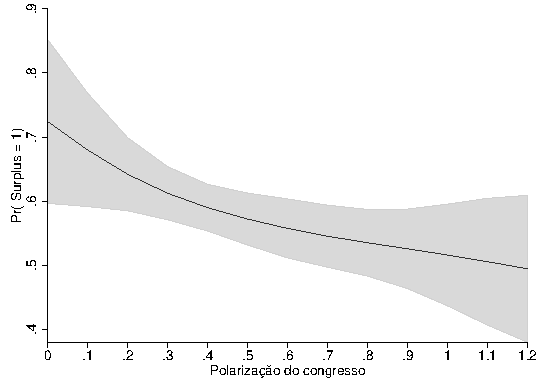
\includegraphics[scale=1.5]{polarization.pdf}
	\end{center}
	\legend{Fonte: elaboração própria.}
\end{figure}


Outra variável de interesse com efeito mais substantivo é o Número Efetivo de Partidos Parlamentares. Como previa a Hipótese 2, congressos com mais partidos aumentam a oferta de parceiros potenciais e permitem aos presidentes explorar problemas coordenativos entre estes. De acordo com o modelo 2, a estimativa deste efeito é considerável e corrobora aquela hipótese: com as demais variáveis na média e $t = 2$, um congresso com NEPP igual a 2 possui 4\% de probabilidade de ter uma coalizão sobredimensionada; já com NEPP igual a 10, a probabilidade aumenta para 34\%. De qualquer modo, como a incerteza nessa estimativa é muito elevada, outra abordagem melhor ilustra esse efeito. Simulando os coeficientes e a matriz de variância-covariância do modelo 2 mil vezes \footnote{Utilizei o conjunto de macros CLARIFY, de Tomz et al., (\citeyear{tomz2003}), para gerar essas quantidades de interesse.}, a distribuição das probabilidades de surgirem coalizões sobredimensionadas quando o NEPP é de 2 e de 10, respectivamente, é apresentada na~\hyperref[fig:figura2]{Figura 2}. Como é possível verificar, a diferença entre a média das estimativas oculta os platôs mais salientes nas extremidades, mais condizentes com a hipótese inicial.

\begin{figure}[htb]
	\label{fig:figura2}
	\caption{Distribuição do efeito do Número Efetivo de Partidos Parlamentares sobre a probabilidade de ocorrência de coalizões sobredimensionadas}
	\begin{center}
	    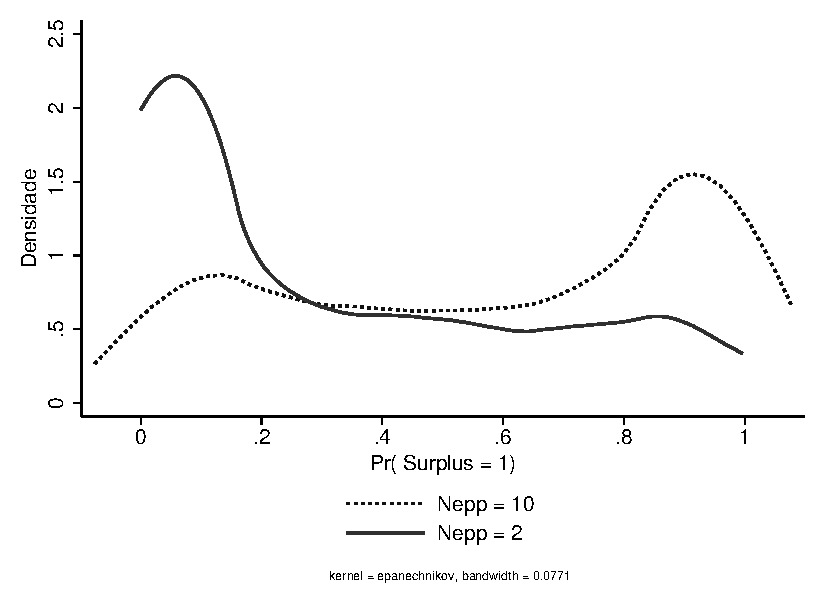
\includegraphics[scale=1.1]{enp.pdf}
	\end{center}
	\legend{Fonte: elaboração própria.}
\end{figure}


Por fim, o efeito da dependência temporal de um ano para outro nos três primeiros modelos merecem um comentário. Quando o gabinete imediatamente anterior é sobredimensionado, a probabilidade de que o corrente também seja é de 65\%, de acordo com o modelo 1. Como seria de se esperar, gabinetes multipartidários frequentemente duram mais do que um ano, mas esse efeito de continuidade desaparece rapidamente: quando a distância temporal entre um gabinete sobredimensionado e outro é maior do que dois anos, a probabilidade deste também ser sobredimensionado é quase 0. Embora não desapareçam repentinamente, portanto, governos com coalizões grandes parecem não durar mais do que um mandato de 4 anos, em média.

Com apenas um indicador binário para captar a presença de coalizões sobredimensionadas, gabinetes com apenas um pequeno partido adicional, como muitos dos formados pela \textit{Concertación}, no Chile, são indistinguíveis de outros com mais partidos. Para contornar isso, os modelos 4 e 5, que empregam o número de partidos excedentes na coalizão como variável dependente. Os principais resultados estão de acordo com os modelos anteriores. O poder presidencial atinge significância, mas, novamente, no sinal oposto ao que previa a Hipótese 3. Fixando as demais variáveis do modelo 4 na média, um presidente com o \textit{score} máximo no índice de poder presidencial aumenta em 0.34 o número esperado de partidos adicionais na coalizão; já utilizando os valores originais da amostra, fixando apenas o valor da variável de interesse, mesmo número chega a quase 1. A~\hyperref[fig:figura3]{Figura 3} exibe este efeito para todos os valores do índice de poder presidencial.

\begin{figure}[htb]
	\label{fig:figura3}
	\caption{Efeito do poder presidencial sobre o número esperado de partidos adicionais na coalizão}
	\begin{center}
	    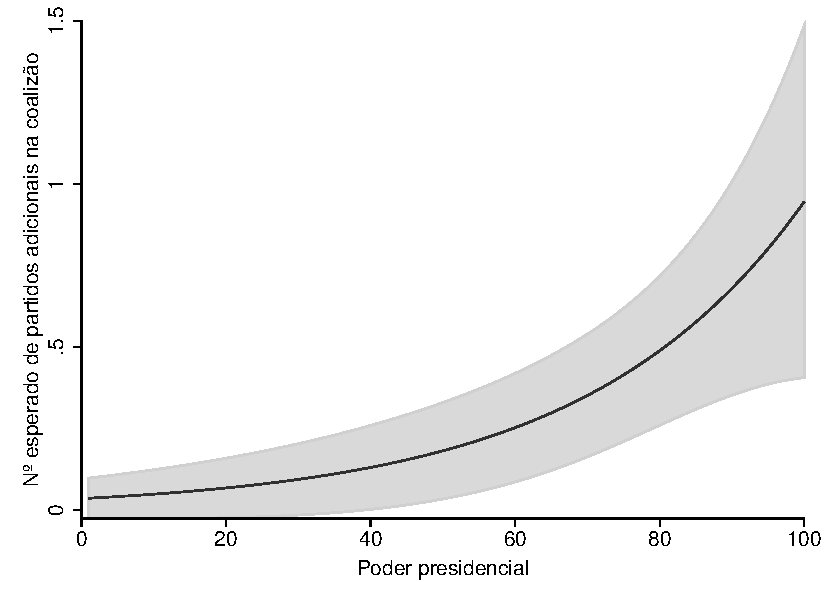
\includegraphics[scale=1]{negretto.pdf}
	\end{center}
	\legend{Fonte: elaboração própria.}
\end{figure}


No modelo 5, Número Efetivo de Partidos Parlamentares mantém o efeito positivo, agora sobre o valor esperado de partidos adicionais na coalizão, e adquire uma estimativa mais precisa. De todo o modo, de acordo com o modelo 5, a mudança de 2 para 10 partidos efetivos gera um aumento esperado de 0.08 partidos adicionais na coalizão, com as demais variáveis fixadas na média. Quanto à efetividade do legislativo, apesar da redução na amostra por ela não estar disponível para todos os casos, a diferença entre o congresso mais efetivo e o menos efetivo é de 0.33 partidos adicionais. Isoladamente, a variável com efeito mais substantivo no modelo 5 continua sendo a polarização no congresso: a maior polarização registrada na amostra provoca um aumento de 0.51 partidos adicionais esperados maior do que o menos polarizados, todo o resto fixo.



\FloatBarrier
\subsection{Testes adicionais}

Para explorar melhor os dados, os Apêndices apresentam os resultados de outros modelos estimados, que incluem operacionalizações alternativas de algumas variáveis, controles adicionais, remoção de alguns países e uso de outras versões da amostra. Embora algumas alterações se verifiquem, os principais resultados apresentados acima se mantêm.